\documentclass{article}
\usepackage{multicol}
\usepackage[english]{babel}
\usepackage{cite}
\usepackage{setspace}
\usepackage{amsmath}
\usepackage{nameref}
\usepackage[round]{natbib}
\usepackage{hyperref}
\usepackage{graphicx}
\usepackage{caption}
\usepackage{subcaption}
\usepackage{amsthm}
\usepackage[utf8]{inputenc}

\usepackage{tikz}
\usetikzlibrary{arrows}

\usepackage{amsthm}
\usepackage{cleveref}

% Page length commands go here in the preamble
\setlength{\oddsidemargin}{-0.25in} % Left margin of 1 in + 0 in = 1 in
\setlength{\textwidth}{7in}   % Right margin of 8.5 in - 1 in - 6.5 in = 1 in
\setlength{\topmargin}{-.75in} % Top margin of 2 in -0.75 in = 1 in
\setlength{\textheight}{9.2in}  % Lower margin of 11 in - 9 in - 1 in = 1 in


\theoremstyle{definition}
\newtheorem{mydef}{Definition}

\usepackage[T1]{fontenc}
\usepackage[utf8]{inputenc}
\usepackage{authblk}

\title{dr-disco intronic}

\author[1]{Youri Hoogstrate}
\affil[1]{Department of Urology, Erasmus University Medical Center}




\begin{document}
\maketitle

%\singlespacing
%	\begin{abstract}\textbf{}
%	\end{abstract}

%	\begin{center}
%	\line(1,0){250}
%	\end{center}
%\newpage
%\tableofcontents
%\newpage

\twocolumn
%\doublespace

\section{Methods}
The tool \textit{dr-disco intronic} tool tries to estimate break points on 2 levels: the exon-exon and the intron-intron boundaries (in case of an intron to intron DNA break point). It takes several steps to accomplish this, described below:

\subsection{Data structure}
The input is an alignment file in the BAM format that specifically contains discordant reads.
Typically those alignments contain aligned reads with an insert sizes that are either too small (overlapping the other mate) or too large (exceeding any reasonable exon length).
The former are typically evidence for local indels or inversions, but seem to occur so often due to library preparation that we deliberately filter them out.
For this we use the criterion that the distance between the aligned reads must at least be 450 ($\sim1.5 \times$ insert size) if they are aligned to the same chromosome.
% Todo: give absolute stats on percentage removal
The remaining reads can either be classified into singletons or paired end reads.
Singletons are reads of which one of the mates was excluded from the alignment while the alignment of the remaining mate was considered discordant.
With BAM/SAM specification it is not possible to describe an inter-chromosomal junction into one single entry.
What is done in RNA-STARs discordant alignment is that discordant reads are being split up into two alignments, of which one is classified as \textit{secondary alignment}.
Because of this the algorithm deals with doubles or triples of aligned reads for singletons and paired end reads respectively.

The main data structure of this application is a \textit{Graph}. There are typically two types of split reads; all singletons are considered to be split reads while paired end reads are only considered split reads if one of the mates is split up.
The remaining mate is then considered a \textit{silent mate} because it only anchors the alignment.
Spanning reads are a double of paired end reads of which none is split up. We classify reads as follows:
\begin{itemize}
	\item Split read
	\begin{itemize}
		\item Singleton aligned chunk 1 \& singleton aligned chunk 2
		\item PE-R1 aligned chunk 1 \& PE-R1 aligned chunk 2 \& silent mate R2
		\item PE-R2 aligned chunk 1 \& PE-R2 aligned chunk 2 \& silent mate R1
	\end{itemize}
	\item Spanning read (double of discordant mates only)
	\begin{itemize}
		\item Paired end R1 read \& Paired end R2 read
	\end{itemize}
	\item Silent mate (triple of discordant mates only)
	\begin{itemize}
		\item PE-R1 aligned chunk 1 \& PE-R1 aligned chunk 2 \& silent mate R2
		\item PE-R2 aligned chunk 1 \& PE-R2 aligned chunk 2 \& silent mate R1
	\end{itemize}
\end{itemize}

According to the subtype and additional information (e.g. strand and clipping flags) the exact junction in the alignment will be determined.
Also, if an aligned chunk contains a splice junction or and indel annotation, this will be considered as a separate type of junction too.
If any of the two positions of a junction does not exist, the position will be inserted into the graph.
When the nodes are all present in the graph, and the edge between the two positions do not exists in the graph, the edge will be inserted (bi-directional) into the graph.
The edge will be annotated such that the weight of the subtype gets increased by one.
The nodes of the graph are also inserted into a genomic-range index (intervaltree-bio python package) to quickly target specific subregions of the graph.
Each node has a property describing the number of (soft/hard)-clips were found in corresponding mates, illustrated in figure \ref{fig:edges_clips}.

\begin{figure}
% xref: http://tex.stackexchange.com/questions/45734/drawing-graphs-in-latex
\begin{tikzpicture}[->,>=stealth',shorten >=1pt,auto,node distance=3cm,
                    thick,main node/.style={circle,draw,font=\sffamily\Large\bfseries}]

  \node[main node] (1) {\small{chr1:100}};
  \node[main node] (2) [right of=1] {\small{chr2:900}};

  \path[every node/.style={font=\sffamily\small}]
    (1) edge [bend left] node {split: 1} (2)
        edge [loop below,color=gray] node {clips: 1} (1)
    (2) edge [bend left] node {split: 1} (1)
        edge [loop below,color=gray] node {clips: 0} (2)
;
\end{tikzpicture}
\caption{Left: graph before pruning, right: after pruning}
\label{fig:edges_clips}
\end{figure}

\subsection{Pruning (the graph)}
Let's assume we have the following alignment, we would like to translate into a graph:
\begin{verbatim}
chr1:
  80        90        100
..|....i....|....i....|....i..
      [----read-01----|
          [--read-02--|
[--read-03--]


chr2:      
       900       910
..i....|....i....|....i....|..
       |--read-01--]
       |----read-02---]
                 [--read-03--]
\end{verbatim}
The corresponding graph would look like presented in figure \ref{fig:pruning_graph} (left).
Hence, in this graph each node is a genomic location and edges represent the junctions in the alignment.
The graph contains two split reads that break from \verb|chr1:100| to \verb|chr2:900| and a spanning read aligned from \verb|chr1:90| to \verb|chr2:910|.
We see that we have actually two very closely adjacent edges; the split and discordant edge differ on both their nodes not more than 10bp.
It is very likely that those two different detected junctions are actually coming from the same genomic event.
Discordant reads do usually not cover the actual break point but are closely adjacent while on the other hand split reads should be falling on the break exactly.
In order to combine this information, this distance of each of the nodes needs to be reasonable, which would mean for the sequencing data that it should not exceed the insert size of the sequencing reads.
Therefore we added the pruning step that merges edges of this type together.

Pruning starts by finding the edge with the highest weight, looking for both its corresponding vertices for arcs that have their edges in no more than the insert size (450bp) away and are in the same orientation.
Because split reads have a higher probability to be exactly on the break point, they have an increased weight for estimating the highest weight.

The data structure of the pruned example is given in figure \ref{fig:pruning_graph} (right).
Although the total weight of all edges stays identical, the number of edges and nodes shall decrease with every pruning operation and the graph shall become smaller in size.
Splice junctions are not taken into account in the pruning function.


\begin{figure*}
% xref: http://tex.stackexchange.com/questions/45734/drawing-graphs-in-latex
\begin{tikzpicture}[->,>=stealth',shorten >=1pt,auto,node distance=3cm,
                    thick,main node/.style={circle,draw,font=\sffamily\Large\bfseries}]

  \node[main node] (1) {\small{chr1:90}};
  \node[main node] (2) [right of=1] {\small{chr1:100}};
  \node[main node] (3) [right of=2] {\small{chr2:900}};
  \node[main node] (4) [right of=3] {\small{chr2:910}};

  \path[every node/.style={font=\sffamily\small}]
    (1) edge [bend left] node {discordant: 1} (4)
%        edge [loop below] node {clips: 0} (4)
    (2) edge [bend left] node {split: 2} (3)
%        edge [loop below] node {clips: 0} (3)
    (3) edge [bend left] node {split: 2} (2)
%        edge [loop below] node {clips: 0} (2)
    (4) edge [bend left] node {discordant: 1} (1)
%        edge [loop below] node {clips: 0} (1)
;
\end{tikzpicture}
\begin{tikzpicture}[->,>=stealth',shorten >=1pt,auto,node distance=3cm,
                    thick,main node/.style={circle,draw,font=\sffamily\Large\bfseries}]

  \node[main node] (1) {\small{chr1:100}};
  \node[main node] (2) [right of=2] {\small{chr2:900}};

  \path[every node/.style={font=\sffamily\small}]
    (1) edge [bend left] node [text width=2cm,align=center]{split: 2, \\ discordant$^*$: 1} (2)
    (2) edge [bend left] node [text width=2cm,align=center]{split: 2, \\ discordant$^*$: 1} (1)
;
\end{tikzpicture}
\caption{Left: graph before pruning, right: after pruning}
\label{fig:pruning_graph}
\end{figure*}

\subsection{Re-joining splice junctions}
The next step is to re-join splice junction(s).
Each splice junction is only present at just two nodes, the boundaries of two exons.
However, if you have a junction on the other side or in the middle of an exon, it is not directly connected to the splice junction.
It is desired to have the exon junctions connected to the junctions.
We would like to include the splice junctions to \textbf{all} edges that are in close proximity (450bp), possibly resulting into one splice junction linking several nodes together.

\begin{verbatim}
thick arcs:
                                ------------------------------------------
                       ---------------------------------------------------
                       ----------------------------------------------------------
              -------------------------------------------------------------------

 splice juncs:
               -------  -------                                            -----
             ||       ||       ||        |          $ ... $       |      ||     ||

        
        the goal is to add the splice juncs between the nodes
\end{verbatim}


\subsection{Extract subnetworks (by splice junctions)}
In the RNA-Seq we find both intronic as exonic break points.
Because intronic break points may be spliced, multiple junctions and thus multiple arcs may contribute to the same fusion gene.
Therefore we would like to take all arcs corresponding to the same junction out of the graph together, just at once.
We then extract subnetworks, sets of 2 nodes and 2 (directional) arcs that are joined by splice junctions.

\subsection{Extract subnetworks}
The complexity is that it may be possible that novel 
Then we merge subnetworks together based on their overall distance to other networks.
This is because it often happens that novel exons are being used or that no splice junctions were present in the alignment.
This may also merge intronic with splice-junction spanning reads.
We apply a filter on the subnetworks that uses the number of discordant reads, split reads and entropy (unique aligned reads in contrast to all reads involved).

The reads spanning the genomic break point are most often not connected by any other read to the reads spanning the nearest splice junctions.
They both end up in a separate 'network' of reads, to be merged afterwards:






\end{document}


